\section{From hourly demand to finite-horizon waiting}
\subsection{Unobserved minute arrivals as explicit scenarios}
Hourly tap-ins do not reveal the minute at which a passenger reaches a platform. For a predicted total $\widehat N_{dsh}$, let $p_{dshm}\geq0$ be the fraction allocated to minute $m\in\{0,\ldots,59\}$, with $\sum_mp_{dshm}=1$. The implied minute mass is
\begin{equation}
A_{dshm}=\widehat N_{dsh}p_{dshm}.
\label{eq:minute}
\end{equation}
The first Beimen experiment compares uniform allocation with truncated broad and concentrated peaks (standard deviations 20 and 5 minutes), alternative peak centers at minute 15, 30 or 45, and directional splits near 40:60, 50:50 and 60:40. Only the model-predicted highest hour receives a nonuniform shape in this early experiment; other hours remain uniform. This is a sensitivity design, \emph{not} an estimate that actual fireworks passengers follow a Gaussian minute profile. A five-minute access-to-platform delay is an assumption rather than a measured distribution.

\subsection{Batch-service queue and passenger-minute identity}
Let $Q_{j-1}$ be passengers left after train $j-1$, $A_j$ new arrivals before train $j$, and $C_j$ the space available to this queue on train $j$. With alighting before boarding, the fluid-count recurrence is
\begin{equation}
Q_j^-=Q_{j-1}+A_j,\qquad
B_j=\min(Q_j^-,C_j),\qquad
Q_j=Q_j^--B_j.
\label{eq:queue}
\end{equation}
This nonnegative conservation law is a train-arrival batch service, not a continuous-service stationary M/M/$c$ queue. If a passenger $\ell$ arrives at minute $a_\ell$ and boards at minute $b_\ell$, while an unserved passenger has $b_\ell>T$, then the total waiting inside horizon $[0,T]$ is
\begin{equation}
W_T=\int_0^T Q(t)\,dt
=\sum_\ell[\min(b_\ell,T)-a_\ell]_+ .
\label{eq:area}
\end{equation}
The equality follows by writing $Q(t)=\sum_\ell \ind\{a_\ell\leq t<\min(b_\ell,T)\}$ and interchanging a finite sum with the integral. It counts only \emph{truncated} waiting for passengers still unserved at $T$. Extending the reference timetable to a common clearing horizon, or reporting residual queues, is necessary before comparing plans. Little's $L=\lambda W$ is a steady-state result \cite{little}; Equation~\eqref{eq:area} is the finite-horizon identity used here.

\subsection{Initial Beimen-only scenario results}
The first study evaluates 1,134 combinations from nine events under the then-current timetable. Remaining space is assumed to be 25\%, 50\% or 75\% of a six-car nominal maximum of 2,220 passengers, corresponding to 555, 1,110 and 1,665 spaces; these are \emph{not} observed carriage loads. Table~\ref{tab:queue} reports event-equal mean waiting after the relevant scenario queues clear. The concentrated peak with only 25\% assumed space produces 7.94 minutes, against 3.39 for a uniform arrival pattern under the same nominal hourly totals. This demonstrates sensitivity to shape and space, not evidence that one shape actually occurred.
\begin{table}[htbp]\centering\small
\caption{Initial Beimen scenario mean waits, minutes; nine events.}
\label{tab:queue}
\begin{tabular}{lrrr}\toprule
Within-hour arrival & 25\% remaining & 50\% remaining & 75\% remaining\\\midrule
Uniform & 3.39 & 3.12 & 3.12\\
Broad peak, SD 20 min & 4.10 & 3.12 & 3.12\\
Concentrated peak, SD 5 min & 7.94 & 4.22 & 3.52\\\bottomrule
\end{tabular}
\end{table}
\begin{figure}[htbp]\centering
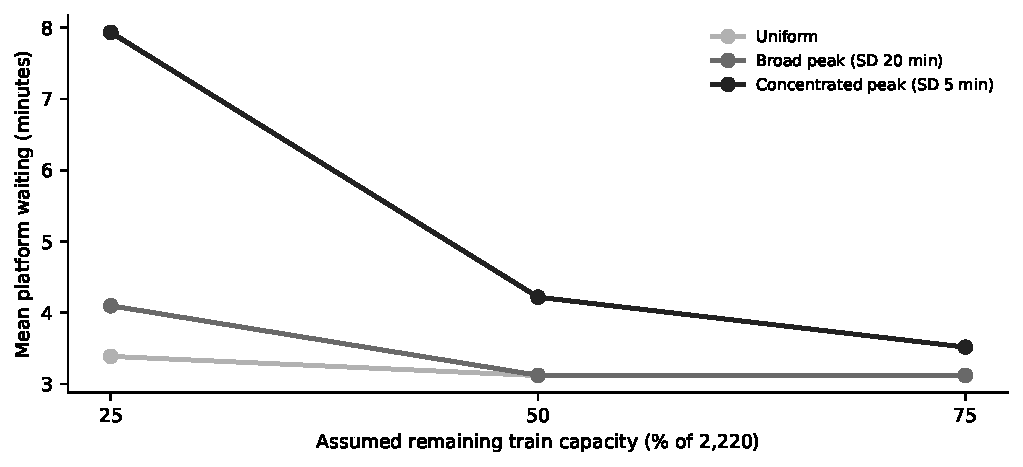
\includegraphics[width=.91\linewidth]{../../result/research_paper/figures/queue_shapes.pdf}
\caption{Conditional Beimen waiting by assumed minute-arrival concentration and remaining train capacity. This single-station experiment must not be numerically pooled with the later full-line model.}
\label{fig:queue}
\end{figure}
\FloatBarrier

\section{Full-line timetable evaluation}
\subsection{Reference schedule, passengers and service feasibility}
The later experiment takes an official Green-line timetable edition as its \emph{reference schedule} and permits add, cancel and retime operations for services whose Beimen departure falls in $[18{:}00,23{:}00)$. Trains outside that decision window and Red/Orange-line schedules are held fixed. Demand from 17:00--18:00 warms the network state; arrivals are injected until 23:00 and fixed later services continue clearing passengers to a common 02:00 terminal horizon. OD-derived trips are assigned by a shortest-time routing proxy; initial platform access and walking transfer time are assumed to be five minutes. Green-line train occupancy follows station-by-station boarding and alighting conservation with a six-car 2,220-person nominal bound. Connecting-line waiting can change when a passenger catches a different service, but full Red/Orange-line on-board capacities are not reconstructed.

Every altered or inserted service is checked against neighboring same-direction services, including those just outside the decision window. A 120-second minimum separation is a \emph{research constraint}, not a verified signaling-safety limit. An admissible solution also requires a finite, cleared waiting calculation in the specified model. Fleet availability, crew, depot departure, turnback, deadhead track conflicts and exact historical event-day train loads are not fully modeled. Thus passing these tests is weaker than being a physically executable operating order.

\subsection{Monetary objective and the meaning of a reference total}
For a candidate timetable $x$, let $N_+(x)$ and $N_-(x)$ be added and cancelled complete service trips after one-to-one matching of retimed trains. At the unverified variable-cost proxy of TWD 128.05 per train-kilometer, one 18.77-km full route plus one \emph{assumed} equal-length empty return for each added service, but only one avoided full-route service for a cancellation, gives
\begin{equation}
\Delta C_{\mathrm{op}}(x)=128.05(18.77)\{2N_+(x)-N_-(x)\}.
\label{eq:opcost}
\end{equation}
The matching prevents a retime from being counted as both a cancellation and an addition. Fixed payroll, depreciation and other unavoidable expenditures are not subtracted when a train is cancelled. The return movement is a cost assumption without separately modeled path capacity, and the train-kilometer proxy has not been verified against operator marginal-cost accounts.

Let $W_r(x)$ denote total passenger-minutes of waiting under training scenario $r$, and let $\gamma\in\{0.5,1,2\}$ represent a preference multiplier. The project uses the 2026 minimum hourly wage of TWD 196 \cite{wage} merely as an illustrative conversion, $v_0=196/60$ TWD per passenger-minute:
\begin{equation}
J_\gamma(x)=\Delta C_{\mathrm{op}}(x)
+\gamma\frac{196}{60}\frac1S\sum_{r=1}^{S}W_r(x),
\qquad x\in\mathcal P.
\label{eq:objective}
\end{equation}
The wage source supports the wage figure, \emph{not} an empirical claim that every passenger values waiting at that wage. $\gamma$ is not learned from operator choices, neural networks or inverse optimization. Monetary waiting is a welfare proxy rather than cash paid by the operator. Comparing operating expenditure separately from $W$ is therefore essential.

The project contains two quantities that could be described informally as a historical scheduling baseline. The older Beimen-oriented \emph{add-only} experiment stored a reference evaluation objective of about TWD 1.968 million over its eight events, under its own horizon, capacity and residual-queue assumptions. The current full Green-line add/cancel/retime experiment instead stores a reference timetable with 852 simulated services, operating proxy TWD 2.048 million and total waiting 6.425 million passenger-minutes over eight events. For $\gamma=1$, its \emph{modeled combined reference objective} is
\begin{equation}
J_1^{\mathrm{ref}}=
2{,}047{,}780.722+\frac{196}{60}(6{,}425{,}026.817)
=23{,}036{,}201.656\ \text{TWD}.
\label{eq:referenceobjective}
\end{equation}
This is the model value for the reference timetable, \emph{not} an observed historical dispatch bill or official net revenue. The older 1.968-million and current 23.036-million objectives have different passenger populations and conventions; they must not be differenced. All results below compare schedules only \emph{within} the current experiment.

\subsection{Candidate generation, selection and independent evaluation}
For each of eight assessable events, 200 simulated training scenarios are generated; the first 12 support proposal and initial screening. Candidate families include the earlier local search and a later 15-minute allocation grid. The 15-minute unit is a \emph{search bin}, not a train headway. The best training candidates from the earlier family remain available when the later family is added. For each $\gamma$, only training scenarios choose the timetable. A separate set of 300 draws evaluates the selected plan and the unaltered reference using paired inputs. These 500 draws are simulated alternatives, not 500 observed festivals. The earliest 2024 event is excluded from this eight-event dispatch test because no earlier comparable forecast-error event is available to construct its uncertainty scenarios.

The candidate set $\mathcal P$ is finite and contains the reference schedule. Therefore, if each candidate produces finite costs and waiting, the minimum of $J_\gamma$ over $\mathcal P$ exists. This is \emph{not} a proof that the heuristic generated all signaling-, fleet- and crew-feasible timetables, nor a proof of global operational optimality. The full statement and proof appear in Appendix~\ref{sec:proofs}.

\section{Timetable results and diagnostics}
\subsection{Eight-event comparison against the reference timetable}
At $\gamma=1$, Table~\ref{tab:dispatch} gives the independently evaluated, scenario-conditional comparison for the current full-line simulation. In total, 496 service trips are added, none are cancelled, and 608 are retimed according to the plan-matching rule. Mean waiting falls from 3.895 to 2.868 minutes (26.4\% fewer passenger-minutes), while modeled variable operating expenditure \emph{increases} by TWD 2,384,271. The selected plan's combined objective is TWD 19,885,398, lower than the reference value in Equation~\eqref{eq:referenceobjective} by TWD 3,150,803. This decrease is not a cash saving: operating expenditure rises, while monetized simulated waiting falls by more.
\begin{table}[htbp]\centering\small
\caption{Independent-scenario full-line comparison at $\gamma=1$. Cost changes are TWD relative to each reference timetable.}
\label{tab:dispatch}
\begin{tabular}{lrrr}\toprule
Event & Add/cancel/retime & Operating cost change & Mean wait: ref.\ $\to$ plan\\\midrule
2024-07-31 & 50/0/87 & +240,350 & 3.38 $\to$ 2.64\\
2024-08-10 & 78/0/65 & +374,946 & 4.67 $\to$ 3.23\\
2025-08-06 & 51/0/83 & +245,157 & 3.38 $\to$ 2.63\\
2025-08-20 & 58/0/88 & +278,806 & 3.38 $\to$ 2.59\\
2025-08-30 & 86/0/59 & +413,402 & 4.67 $\to$ 3.11\\
2026-07-25 & 56/0/68 & +269,192 & 4.64 $\to$ 3.35\\
2026-08-05 & 57/0/87 & +273,999 & 3.36 $\to$ 2.59\\
2026-08-15 & 60/0/71 & +288,420 & 4.64 $\to$ 3.31\\\midrule
Eight-event total/weighted mean & 496/0/608 & +2,384,271 & 3.89 $\to$ 2.87\\\bottomrule
\end{tabular}
\end{table}

The preference sensitivity in Table~\ref{tab:weightsensitivity} makes the operating--waiting trade-off explicit. Higher $\gamma$ increases the value assigned to saved waiting and hence selects more service in these candidates; it does not mean that the higher setting is empirically or ethically correct. The monetary objectives at different $\gamma$ values are not on a common preference scale and should not be ranked to estimate $\gamma$.
\begin{table}[htbp]\centering\small
\caption{Eight-event sensitivity to the illustrative waiting-value multiplier.}
\label{tab:weightsensitivity}
\begin{tabular}{rrrrr}\toprule
$\gamma$ & Added & Cancelled & Operating change (TWD) & Mean wait (min)\\\midrule
0.5 & 169 & 0 & +812,382 & 3.308\\
1.0 & 496 & 0 & +2,384,271 & 2.868\\
2.0 & 1,069 & 0 & +5,138,680 & 2.527\\\bottomrule
\end{tabular}
\end{table}
\begin{figure}[htbp]\centering
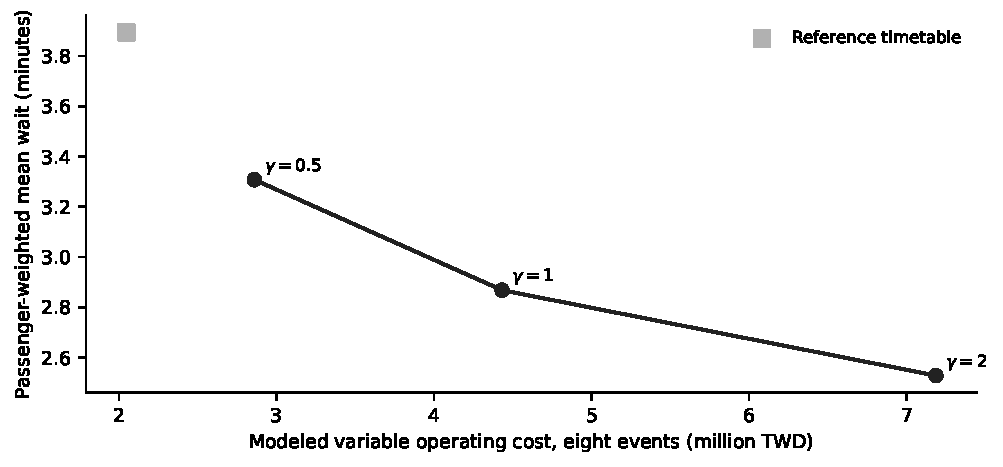
\includegraphics[width=.90\linewidth]{../../result/research_paper/figures/dispatch_tradeoff.pdf}
\caption{Modeled operating expenditure and waiting for the reference timetable and three selected preference scenarios. These are finite candidates, not a complete Pareto frontier.}
\label{fig:tradeoff}
\end{figure}

\subsection{Why cancellation was not selected}
A follow-up decomposition uses the \emph{same} eight-event, $\gamma=1$ selected plans and evaluation draws. Of the 1,694,410 passenger-minutes of modeled waiting reduction, 234,087 (13.8\%) belong to Beimen-classified journeys, 59,699 (3.5\%) to the other three study-station classes, and 1,400,624 (82.7\%) to other modeled passengers on the line. These are mutually assigned model groups, not measured counts of real passenger preferences. The large background group can make additional trains attractive in an all-passenger objective even if a Beimen-only criterion would choose differently. Early screening may also favor dense service; the decomposition is a diagnostic, not a proof that cancellation is never optimal.
\begin{figure}[htbp]\centering
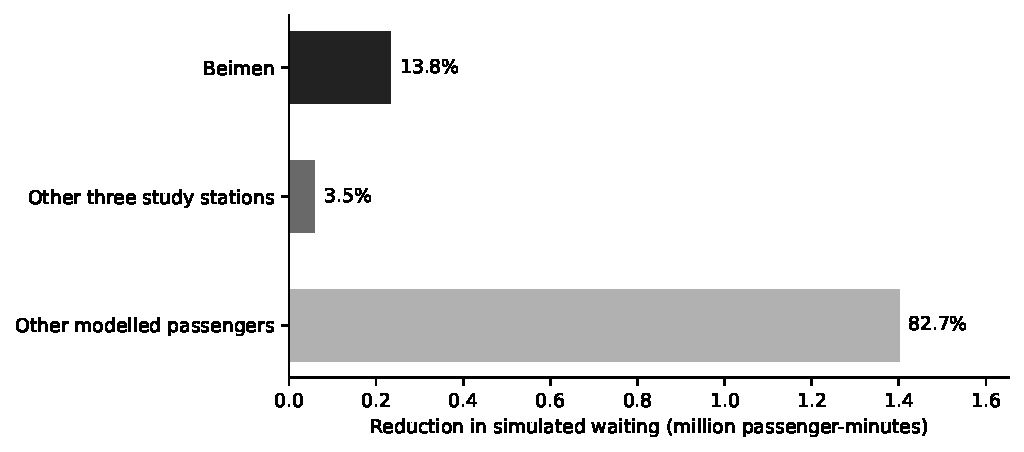
\includegraphics[width=.90\linewidth]{../../result/research_paper/figures/benefit_split.pdf}
\caption{Source of simulated waiting reduction for the selected $\gamma=1$ timetable, eight events combined. The background group is model-generated.}
\label{fig:benefit}
\end{figure}
Equation~\eqref{eq:opcost} makes cancellation of one full-route service worth approximately $c_-=128.05(18.77)=2{,}403.50$ TWD before waiting is counted. If all other decisions are fixed, cancellation is favorable at $\gamma=1$ only when the resulting increase in total expected waiting is below $c_-/(196/60)=735.76$ passenger-minutes. Multiple simultaneous changes can interact, so this is a local, conditional break-even calculation. A negative 15-minute heatmap cell is not itself a cancelled trip: retiming a service across adjacent grid cells also creates a negative and a positive cell.
\FloatBarrier

\subsection{Unknown train loading and operational validity}
Train free space in the later simulation is propagated from OD-derived flows, timetables and assumed routes. This is a meaningful improvement over assuming that every passing train has exactly 50\% free space, but it is \emph{not} a calibration to measured eight-event vehicle loads. A crowding-level API is a potential data-access lead \cite{crowding}; categorical live levels do not reconstruct historical numeric loads for the studied trains. If available space is systematically overestimated, simulated queues and the demand for extra trains will be understated; underestimation can yield excessive additional service. The most consequential next empirical input is matched train occupancy and minute-level platform/gate arrivals, followed by actual historical service and dispatch records.
